\section{A Performance Model for \headershortacr{3G} \headershortacr{RRC} States}\label{sec:network:performance_model}
\cite{Schwartz2013c}

\subsection{System Description and Basic Assumptions}\label{sec:network:performance_model:system_description}
\begin{figure}
	\begin{subfigure}[b]{.5\textwidth}
	\centering
	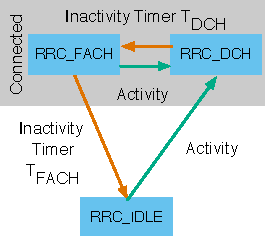
\includegraphics{network/background/figures//three_states}
	\caption{Three State Scenario}\label{fig:network:background:rrc_state_machines:three_states}
	\end{subfigure}%
	\begin{subfigure}[b]{.5\textwidth}
	\centering
	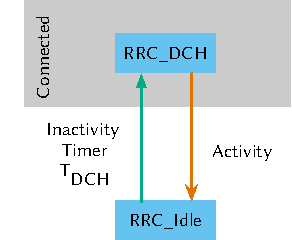
\includegraphics{network/background/figures//two_states}
	\caption{Two State Scenario}\label{fig:network:background:rrc_state_machines:two_states}
	\end{subfigure}
	\caption{\headershortacr{RRC} State Machine Diagrams}\label{fig:network:background:rrc_state_machines}
\end{figure}

\subsubsection*{The Case of Two \headershortacr{RRC} States}\label{sec:network:performance_model:system_description:two_states}
\subsubsection*{Extension for Three \headershortacr{RRC} States}\label{sec:network:performance_model:system_description:three_states}
\subsubsection*{Modeling Signaling Intensity and Power Drain of the \headershortacr{UE}}\label{sec:network:performance_model:system_description:metrics}

\subsection{Numerical Examples and Their Implications}\label{sec:network:performance_model:numerical_examples}
\subsubsection*{Model Validations}\label{sec:network:performance_model:validations}
\subsubsection*{Impact of Traffic Patterns on Signaling Intensity}\label{sec:network:performance_model:signaling_intensity}
\subsubsection*{Impact of Traffic Patterns on Power Drain of the \headershortacr{UE}}\label{sec:network:performance_model:power_drain}
\subsubsection*{Trade-off: Energy Consumption vs. Signalling Load}\label{sec:network:performance_model:trade_off}
